\documentclass{article}
\usepackage[landscape, margin=4mm, paper=a6paper, includehead, includefoot]{geometry}
\usepackage{lipsum}
\usepackage{graphicx}
\usepackage{multicol}
\usepackage{fancyhdr}
\usepackage{scrextend}
\usepackage{paralist}

\KOMAoptions{fontsize=8pt}
\setlength{\parindent}{0pt}
\raggedright

% Define fancy headers and footers
\pagestyle{fancy}
\fancyhf{}
\fancyhead[L]{\leftmark}
\fancyfoot[C]{\thepage}


%%%%%%%%%%%%% DOCUMENT START %%%%%%%%%%%%%
\begin{document}
\pagenumbering{gobble}

%%%%%%%%%%%%% FIRST PAGE %%%%%%%%%%%%%
% \newpage
% % HEADER:
% \pagestyle{fancy}
% \fancyhf{}                    %%%% REMOVING PRIOR HEAD AND FOOT
% \fancyhead[L]{GMT}            %%%% HEAD LEFT SUBJECT
% \fancyhead[C]{Werkstoffe-Main}     %%%% HEAD MID TOPIC
% \fancyhead[R]{Holz, Ökologie} %%%% HEAD RIGHT SUBTOPIC

% CONTENT START
% \paragraph{Warum kann die Holzgewinnung ökologisch bedenklich sein?}
% \begin{itemize}
% \item Trotz der Tatsache, dass Holz ein nachwachsender Rohstoff ist, kann die
  % Holzgewinnung problematisch sein. Beispiele hierfür sind übermäßige
  % Abholzung, versäumte Wiederaufforstung, Plantagenwirtschaft in Monokulturen
  % oder Bodenverdichtung. Insbesondere bei Tropenhölzern kann die Abholzung der
  % Regenwälder oder die Holzgewinnung für die Papierindustrie durch Abholzen der
  % großen kanadischen Urwälder ökologisch bedenklich sein.
% \end{itemize}
% FOOTER:
% \fancyfoot[L]{Daniel Renschler}
% \fancyfoot[R]{J1-2}



% TEMPLATES:
%%%%%%%%%%%%% personal %%%%%%%%%%%%%
%\newpage
% HEADER:
%\pagestyle{fancy}
%\fancyhf{}                    %%%% REMOVING PRIOR HEAD AND FOOT
%\fancyhead[L]{subject}            %%%% HEAD LEFT SUBJECT
%\fancyhead[C]{topic}     %%%% HEAD MID TOPIC
%\fancyhead[R]{subtopic}         %%%% HEAD RIGHT SUBTOPIC

%TITLE:
%\paragraph{title}
%CONTENT START
%\begin{itemize}
%\item content%CONTENT AS ITEM
%\end{itemize}

% FOOTER:
%\fancyfoot[L]{Daniel Renschler}
%\fancyfoot[R]{J1-2}


%%%%%%%%%%%%%%%%%% VARIABLE CARD %%%%%%%%%%%%%%%%%%%%%%%%%%TESTTESTSETTESSETSETSETSETSETSET%%%%%%%%%%%%%%%%%%%%%%%%%%%%
\newpage
% HEADER:
\pagestyle{fancy}
\fancyhf{}                    %%%% REMOVING PRIOR HEAD AND FOOT
\fancyhead[L]{GMT}        %%%% HEAD LEFT SUBJECT
\fancyhead[C]{Werkstoffe}          %%%% HEAD MID TOPIC
\fancyhead[R]{Aluminium}       %%%% HEAD RIGHT SUBTOPIC

% TESTING MULTICOL
\begin{multicols}{3}
\paragraph{Aluminium:}

\includegraphics[width=\linewidth]{alu.jpg}
\paragraph{Allgemeine Informaionen}
Dichte: 2,7$\frac{g}{cm^3}$\\
Zugfestigkeit: 60-600 $\frac{N}{mm^2}$, flach.\\
Schmelzpunkt 660°C
\begin{compactitem}
  \item weich/zähes Metall
  \item gut biegbar (Alu. Druckguss)
\end{compactitem}

Gewonnen durch Elektrolyse pro 1t Alu entstehen 1,6-3,7t giftiger roter Schlamm.

Leicht zu verarbeiten im Vergleich zu anderen Metallen (wenig Energie Notwendig).

\paragraph{Verwertung:}
\begin{compactitem}
  \item sehr gut recylcebar
  \item 75\% werden recycelt
  \item $\to$ dabei nur 10\% wie bei der Erzeugung notwendig.
\end{compactitem}

\paragraph{Depinierung:}
\begin{compactitem}
  \item zersetzt sich kaum.
\end{compactitem}

\paragraph{Warum ist es wichtig?}
\begin{compactitem}
  \item gut leitbar
  \item oft in legierungen
  \item Leicht
  \item korrosions resistent
\end{compactitem}

\paragraph{Verwendung:}
\begin{compactitem}
  \item Architektur
  \item Elektrische Geräte
  \item Transportation
\end{compactitem}



\end{multicols}

\fancyfoot[L]{Daniel Renschler}
\fancyfoot[R]{J1-2}

%%%%%%%%%%%%%%%%%%%%%%%%%%%%%%%%%%%%%%%%%%%%%%%%%%
\newpage
% HEADER:
\pagestyle{fancy}
\fancyhf{}                    %%%% REMOVING PRIOR HEAD AND FOOT
\fancyhead[L]{GMT}        %%%% HEAD LEFT SUBJECT
\fancyhead[C]{Werkstoffe-Main}          %%%% HEAD MID TOPIC
\fancyhead[R]{Stähle}       %%%% HEAD RIGHT SUBTOPIC


% TESTING MULTICOL
%\vspace{-10mm}
\begin{multicols}{3}
  \paragraph{Stahl:}
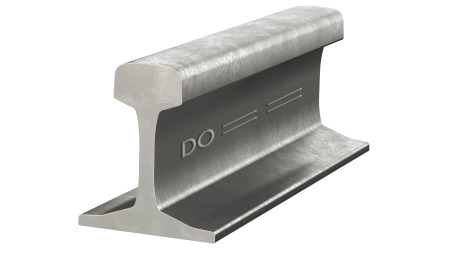
\includegraphics[width=\linewidth]{stahl.jpg}
\paragraph{Allgemeine Informaionen}
Dichte: 7,8-7,9 $\frac{g}{cm^3}$\\
Zugfestigkeit: 290-1270 $\frac{N}{mm^2}$ hohe Varianz wegen unterschied in Baustahl und Vergütungsstahl.\\
Schmelzpunkt: 1550°
\begin{compactitem}
  \item magnetisch
  \item je nach sorte gut giesbar
  \item umformbar
  \item spannbar
  \item Änderungen der Stoffeigenschaften
\end{compactitem}


\begin{compactitem}
  \item Abbau untertage mit Kohle
  \item Schmelzung im Hochofen
  \subitem $\to$ großer Energieufwand durch hohe temp.
  \item Energieaufwand bei bearbeitung hoch, da es meist glühen muss.
  \item Rostet (außer rostfreier Stähle)
  \subitem $\to$ Korrosionsschutz benötigt
\end{compactitem}

\paragraph{Verwertung:}
\begin{compactitem}
  \item gut einschmelzbar
  \item recycling quote fast 100\%
  \item 40\% von Herstellungsenergie notwenig wegen hohem Schmelzpunkt von 1550°C
\end{compactitem}

\paragraph{Entsorgung:}
\begin{compactitem}
  \item Rostet langsam
\end{compactitem}

\paragraph{Warum ist es wichtig?}
\begin{compactitem}
  \item wichtigster Baustoff
  \item recyclebar
  \item fest
  \item gute Leitfähigkeit
  \subitem $\to$ Wärme \& Strom
\end{compactitem}

\paragraph{Beispiele}
\begin{compactitem}
  \item Architektur
  \item Autos
  \item Flugzeuge
  \item Elektronik Geräte
\end{compactitem}
\end{multicols}


\fancyfoot[L]{Daniel Renschler}
\fancyfoot[R]{J1-2}
\clearpage

%%%%%%%%%%%%%%%%%% KUPFERLEGIERUNG %%%%%%%%%%%%%%%%%%%%%%
\newpage
% HEADER:
\pagestyle{fancy}
\fancyhf{}
\fancyhead[L]{GMT}
\fancyhead[C]{Werkstoffe-Main}
\fancyhead[R]{Kupferlegierung}

%\vspace{-10mm}
\begin{multicols}{3}

\paragraph{Kupferlegierung:}
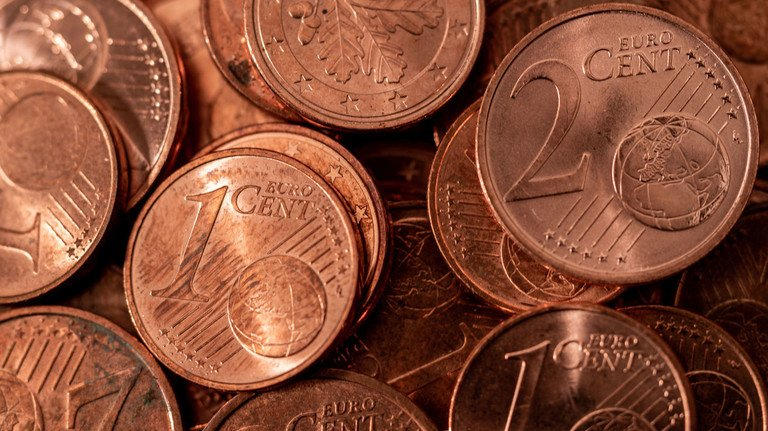
\includegraphics[width=\linewidth]{copper.jpg}
\paragraph{Allgemeine Informaionen} Dichte: Die Dichte von Kupferlegierungen
variiert je nach Legierung und beträgt im Allgemeinen zwischen 7,7 und 8,8 $\frac{g}{cm^3}$.

Zugfestigkeit: Die Zugfestigkeit von Kupferlegierungen hängt von der genauen
Legierung ab. Beispielsweise hat eine typische Messinglegierung eine
Zugfestigkeit von etwa 350 MPa.

Aus was ist es hergestellt? Kupferlegierungen werden aus einer Mischung von
Kupfer und anderen Metallen hergestellt, um bestimmte Eigenschaften wie Härte,
Festigkeit, Korrosionsbeständigkeit und elektrische Leitfähigkeit zu erzielen.
Beispiele für Kupferlegierungen sind Messing (Kupfer und Zink), Bronze (Kupfer
und Zinn) und Kupfer-Nickel-Legierungen.

Wie ist es hergestellt? Kupferlegierungen werden durch Schmelzen der
Ausgangsmetalle und Mischen in einem Ofen hergestellt. Die Legierung wird dann
in eine Form gegossen und abgekühlt, um ein fertiges Produkt zu erhalten.

\paragraph{Verwendung:}
\begin{compactitem}
\item Kupferlegierungen werden in einer Vielzahl von Anwendungen eingesetzt,
  darunter Elektrotechnik, Bauwesen, Schmuckherstellung, Automobilindustrie,
  Luft- und Raumfahrtindustrie sowie in der Lebensmittelindustrie.
\end{compactitem}

\paragraph{Verwertung:}
\begin{compactitem}
\item Kupferlegierungen können durch Recycling wiederverwendet werden. Das
  Recycling von Kupferlegierungen spart Energie und Ressourcen im Vergleich zur
  Herstellung von neuen Kupferlegierungen aus Rohstoffen.
\end{compactitem}

\paragraph{Entsorgung:}
\begin{compactitem}
\item Kupferlegierungen können als Altmetall entsorgt werden. Recycling ist
  jedoch die bevorzugte Methode, da es dazu beiträgt, die Umweltauswirkungen zu
  minimieren.
\end{compactitem}

\paragraph{Warum ist es wichtig?}
\begin{compactitem}
\item Kupferlegierungen sind aufgrund ihrer einzigartigen Kombination aus
  Eigenschaften wie Festigkeit, Härte und Korrosionsbeständigkeit in vielen
  Industriezweigen unverzichtbar. Darüber hinaus ist Kupfer eine hervorragende
  elektrische Leitfähigkeit, was es zu einem wichtigen Material in der
  Elektrotechnik macht.
\end{compactitem}

\paragraph{Beispiele}
\begin{compactitem}
\item Beispiele für die Verwendung von Kupferlegierungen sind elektrische Kabel
  und Leitungen, Rohre, Schmuck, Münzen, Armaturen, elektronische Bauteile und
  Turbinen in der Energieerzeugung. Kupferlegierungen werden auch in der
  Medizintechnik eingesetzt, beispielsweise für Implantate und Instrumente. In
  der Bauindustrie werden Kupferlegierungen für Dächer, Fassadenverkleidungen
  und Wasserleitungen verwendet. In der Automobilindustrie werden
  Kupferlegierungen für Bremsleitungen und Kühlsysteme verwendet. In der Luft-
  und Raumfahrtindustrie werden Kupferlegierungen für Strahltriebwerke,
  Raumfahrzeuge und Flugzeuge verwendet.en in der Energieerzeugung.
  Kupferlegierungen werden auch in der Medizintechnik eingesetzt,
  beispielsweise für Implantate und Instrumente. In der Bauindustrie werden
  Kupferlegierungen für Dächer, Fassadenverkleidungen und Wasserleitungen
  verwendet. In der Automobilindustrie werden Kupferlegierungen für
  Bremsleitungen und Kühlsysteme verwendet. In der Luft- und Raumfahrtindustrie
  werden Kupferlegierungen für Strahltriebwerke, Raumfahrzeuge und Flugzeuge
  verwendet.
\end{compactitem}

\end{document}
